\documentclass[fleqn]{beamer}
\beamertemplatenavigationsymbolsempty

\usepackage[T1]{fontenc}
\usepackage[utf8]{inputenc}

\usepackage{amsmath,amssymb}
\usepackage{nccmath}
\usepackage{graphicx}
\usepackage{mathptmx}
\usepackage{mathtools}
\usepackage{subcaption}
\usepackage{amsthm}
\usepackage{tikz}
\usepackage{pgfplots}
%\usepackage[colorlinks=true,naturalnames=true,plainpages=false,pdfpagelabels=true]{hyperref}
\usetikzlibrary{patterns,decorations.pathmorphing,positioning, arrows, chains}

\usepackage[backend=biber, sorting=none]{biblatex}
\addbibresource{uni.bib}

\setbeamertemplate{endpage}{%
    \begin{frame}
        \centering
        \Large \emph{Thank You!}
    \end{frame}
}

\AtEndDocument{\usebeamertemplate{endpage}}

% vertical separator macro
\newcommand{\vsep}{
  \column{0.0\textwidth}
    \begin{tikzpicture}
      \draw[very thick,black!10] (0,0) -- (0,7.3);
    \end{tikzpicture}
}
\setlength{\mathindent}{0pt}

% Beamer theme
\usetheme{UniVienna}
\usefonttheme[onlysmall]{structurebold}
\mode<presentation>
\setbeamercovered{transparent=10}

\title
{Seminar Complex Network Analysis}
\subtitle{Project Progress}
\author[Popović Milutin]
{Popović Milutin}
\date{13. May 2021}

\begin{document}
    \begin{frame}
        \titlepage
    \end{frame}

    \begin{frame}
        \centering
        \textbf{Python Package Dependency Network}
        \vspace{1cm}
        \begin{columns}[T]
            \column{0.4\textwidth}
            \column{0.4\textwidth}
        \end{columns}
    \end{frame}

    \begin{frame}
        \frametitle{Graph}
        \begin{itemize}
            \item directed Graph with approx. $10^{6}$ links and
                $3.6\cdot10^{5}$ nodes
            \item packages represent nodes
            \item dependencies between packages represent links
        \end{itemize}
        \vspace{1cm}
            \centering package1 $\rightarrow$ package2\\
        \vspace{0.25cm}
            \centering only if package1 is dependent on package2
    \end{frame}

    \begin{frame}
        \frametitle{Data}
        \begin{itemize}
            \item data is indexed on PyPI\cite{pypi} (Python Package Index)
            \item \texttt{json}-type for all packages
            \item containing information such as release date, package
                dependencies, download counts
            \item can be resorted into a time evolving network
        \end{itemize}
    \end{frame}

    \begin{frame}
        \frametitle{Analysis}
        \begin{figure}[htpb]
            \centering
            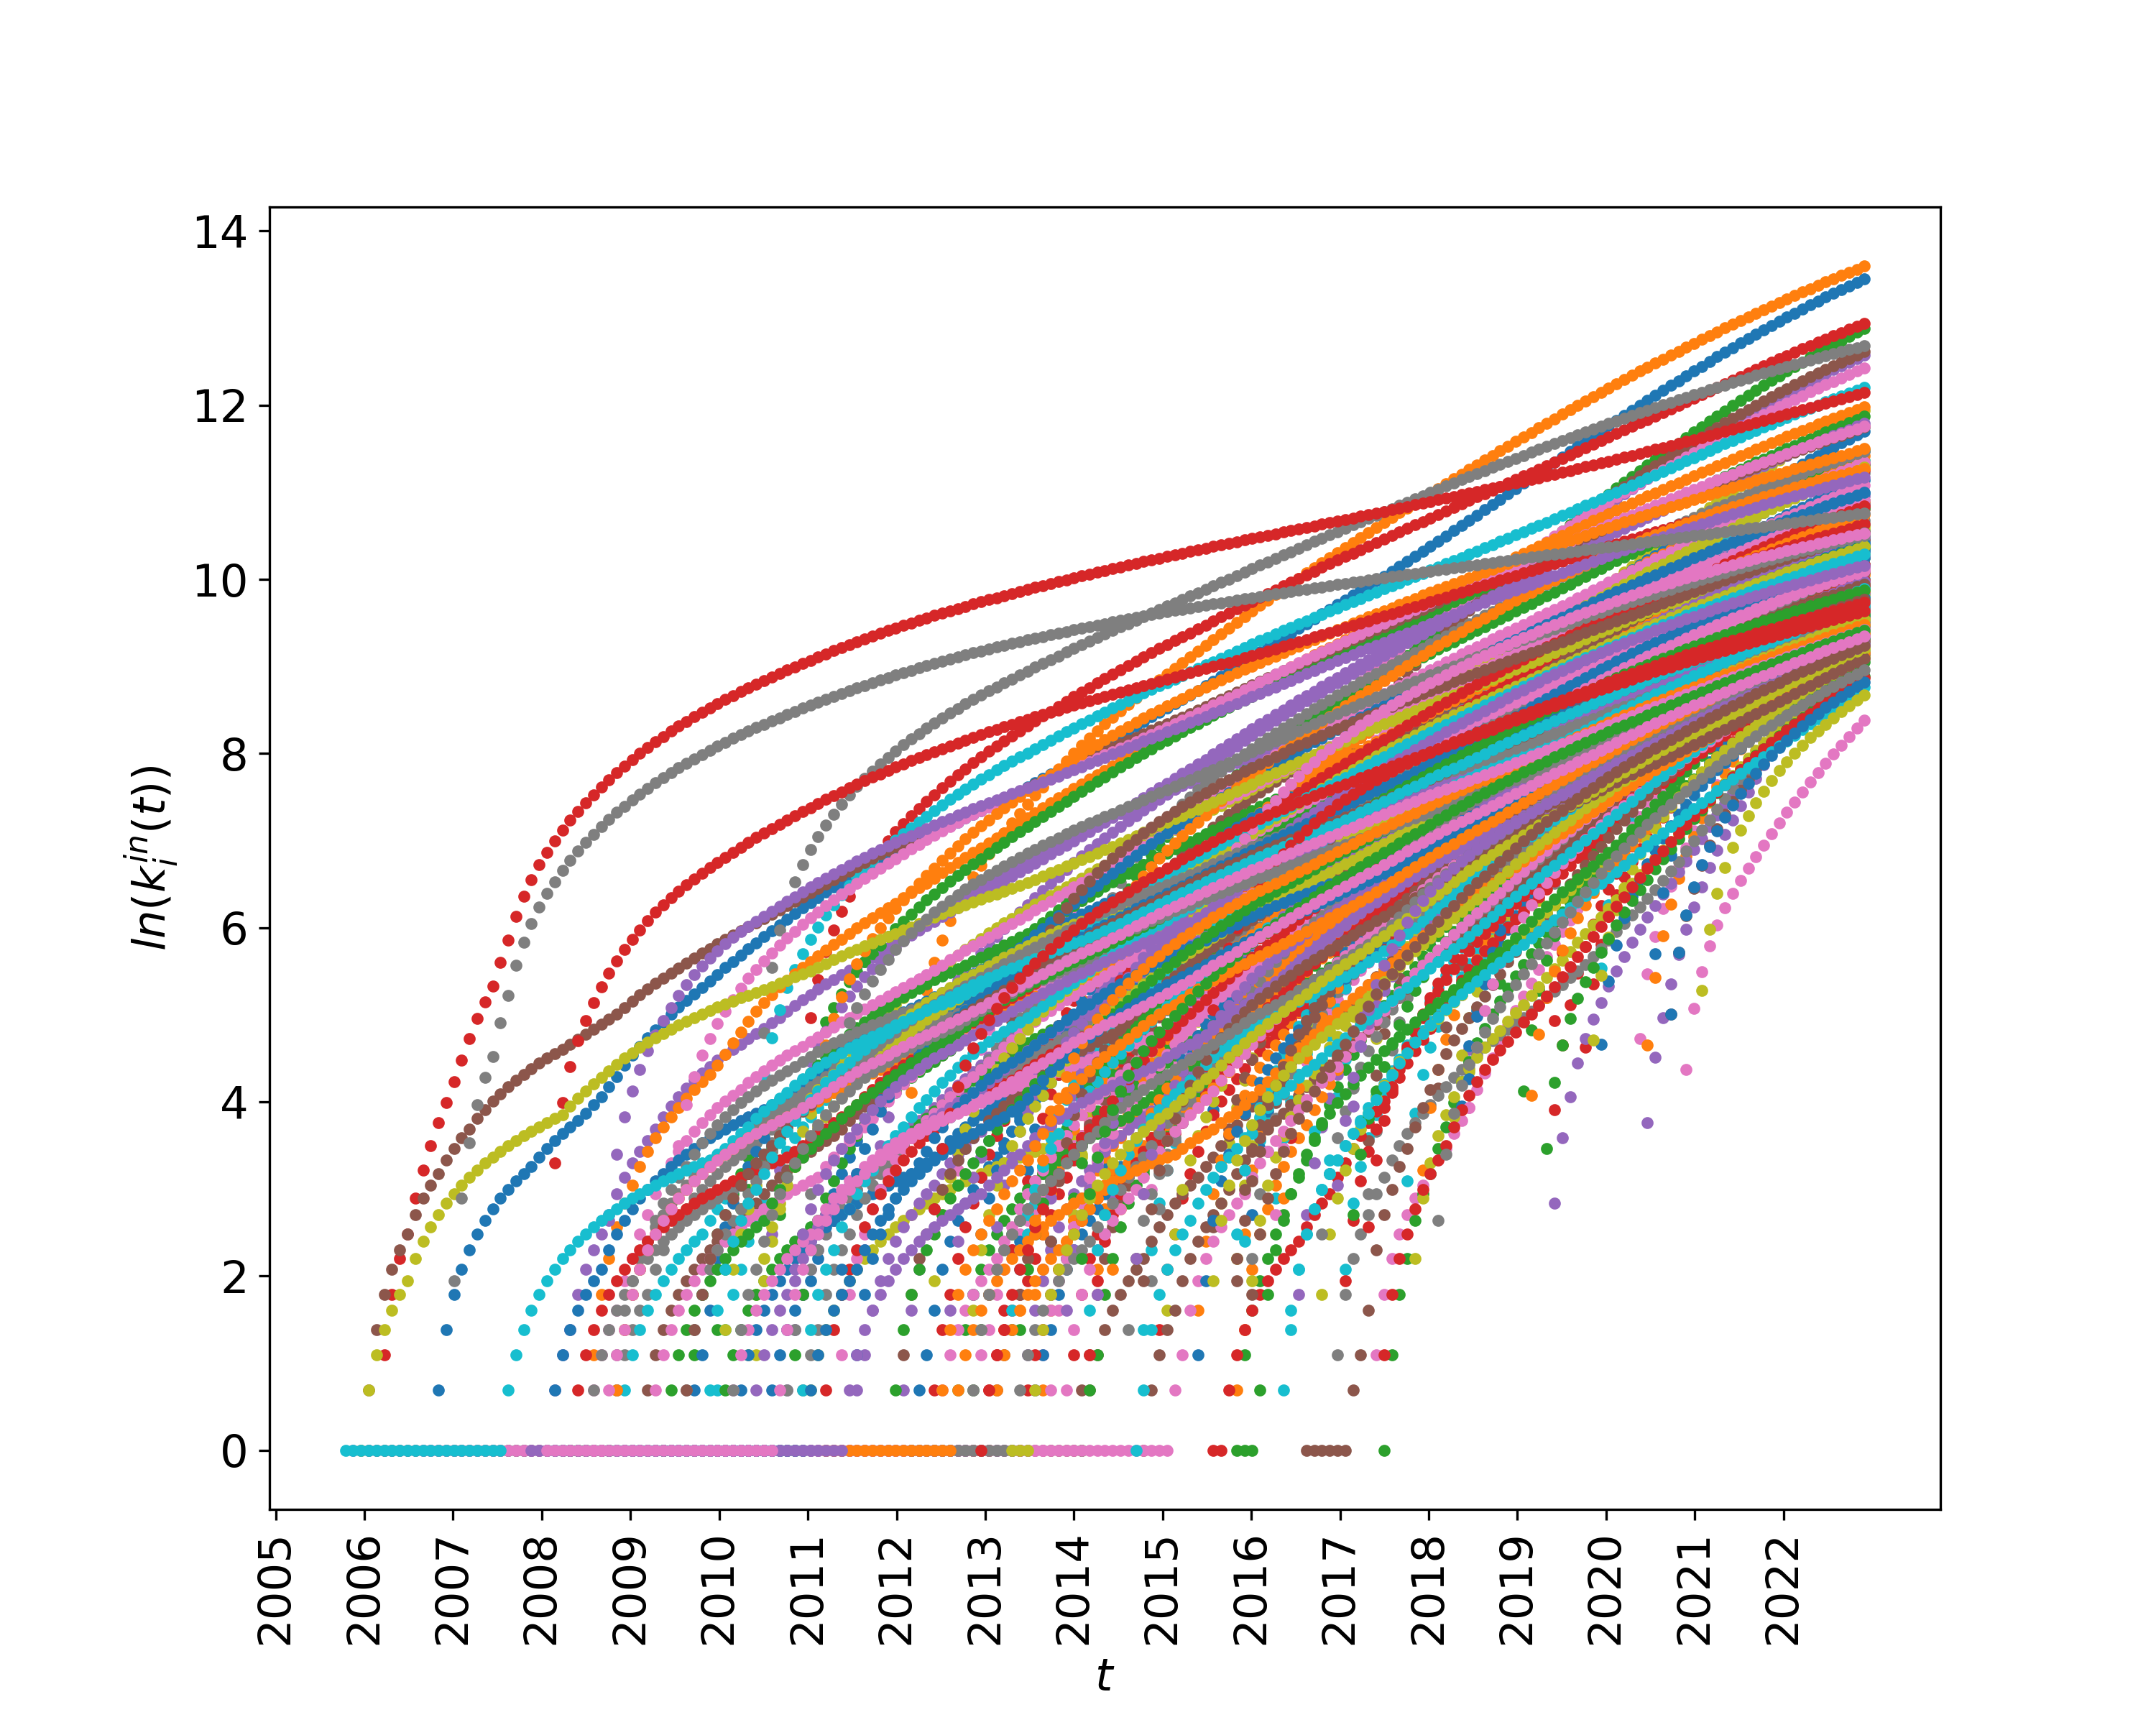
\includegraphics[width=0.8\textwidth]{./pics/top_all_edge_growth.png}
            \caption{Node growth in log scale, all rounder top nodes of all
            time}
        \end{figure}
    \end{frame}

    \begin{frame}
        \frametitle{Analysis since 20016}
        \begin{figure}[htpb]
            \centering
            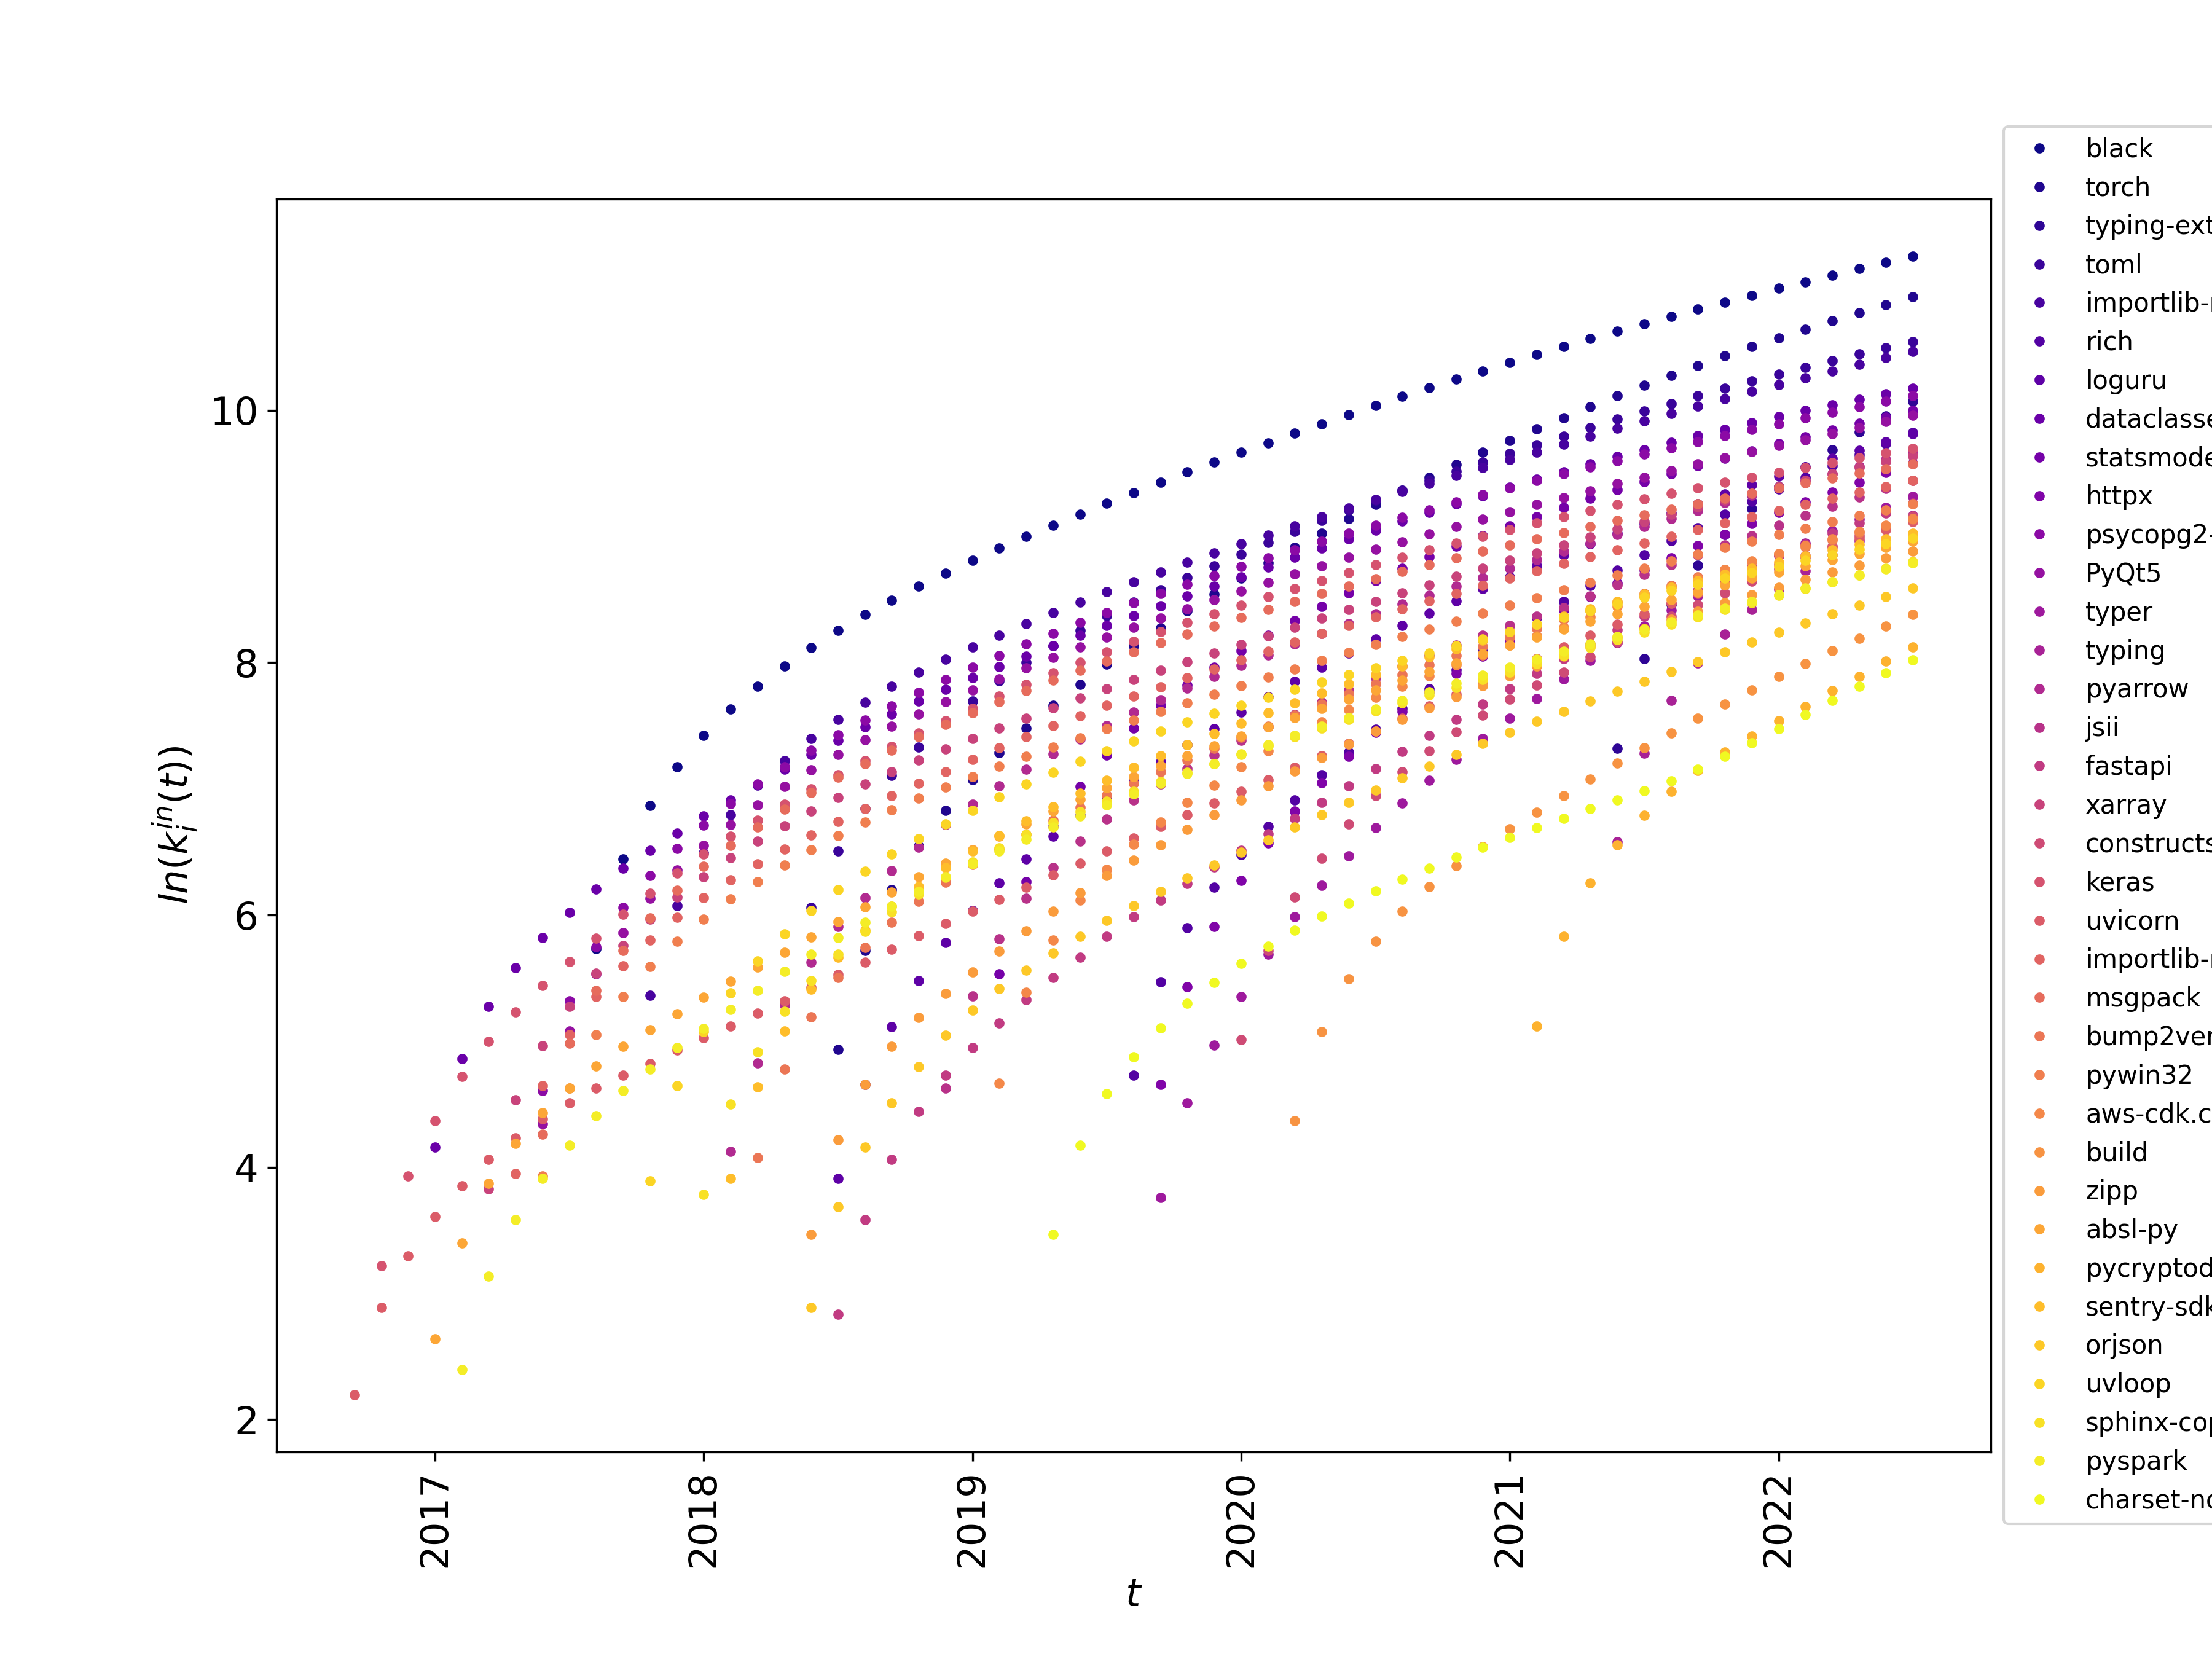
\includegraphics[width=0.8\textwidth]{./pics/deg_2016_growth.png}
        \end{figure}
    \end{frame}

    \begin{frame}
        \frametitle{Visualization}
        \begin{itemize}
            \item Objective: construct a layout to visualize the analysis
                intuitively
            \item layout based on degree distribution (power-law)
        \end{itemize}

        \begin{figure}[htpb]
            \centering
            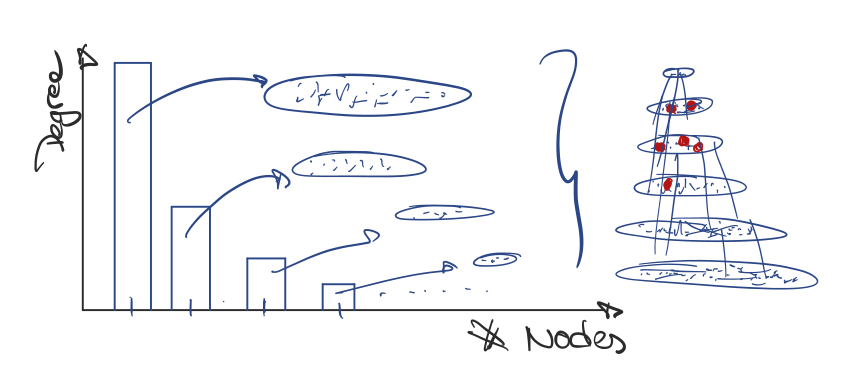
\includegraphics[width=0.8\textwidth]{./pics/layout_setup.png}
            \caption{Layout setup}
        \end{figure}
    \end{frame}
    \begin{frame}
        \frametitle{Outlook}
        \begin{itemize}
            \item incorporate number of downloads into the network
            \item create a weighted directed graph
            \item could open doors to more analysis
        \end{itemize}
    \end{frame}

        \begin{frame}{Bibliography}
            \nocite{barabasi}
            \nocite{pypi}
            \printbibliography
        \end{frame}
\end{document}

